% Options for packages loaded elsewhere
\PassOptionsToPackage{unicode}{hyperref}
\PassOptionsToPackage{hyphens}{url}
%
\documentclass[
  man,floatsintext]{apa6}
\usepackage{amsmath,amssymb}
\usepackage{lmodern}
\usepackage{iftex}
\ifPDFTeX
  \usepackage[T1]{fontenc}
  \usepackage[utf8]{inputenc}
  \usepackage{textcomp} % provide euro and other symbols
\else % if luatex or xetex
  \usepackage{unicode-math}
  \defaultfontfeatures{Scale=MatchLowercase}
  \defaultfontfeatures[\rmfamily]{Ligatures=TeX,Scale=1}
\fi
% Use upquote if available, for straight quotes in verbatim environments
\IfFileExists{upquote.sty}{\usepackage{upquote}}{}
\IfFileExists{microtype.sty}{% use microtype if available
  \usepackage[]{microtype}
  \UseMicrotypeSet[protrusion]{basicmath} % disable protrusion for tt fonts
}{}
\makeatletter
\@ifundefined{KOMAClassName}{% if non-KOMA class
  \IfFileExists{parskip.sty}{%
    \usepackage{parskip}
  }{% else
    \setlength{\parindent}{0pt}
    \setlength{\parskip}{6pt plus 2pt minus 1pt}}
}{% if KOMA class
  \KOMAoptions{parskip=half}}
\makeatother
\usepackage{xcolor}
\usepackage{graphicx}
\makeatletter
\def\maxwidth{\ifdim\Gin@nat@width>\linewidth\linewidth\else\Gin@nat@width\fi}
\def\maxheight{\ifdim\Gin@nat@height>\textheight\textheight\else\Gin@nat@height\fi}
\makeatother
% Scale images if necessary, so that they will not overflow the page
% margins by default, and it is still possible to overwrite the defaults
% using explicit options in \includegraphics[width, height, ...]{}
\setkeys{Gin}{width=\maxwidth,height=\maxheight,keepaspectratio}
% Set default figure placement to htbp
\makeatletter
\def\fps@figure{htbp}
\makeatother
\setlength{\emergencystretch}{3em} % prevent overfull lines
\providecommand{\tightlist}{%
  \setlength{\itemsep}{0pt}\setlength{\parskip}{0pt}}
\setcounter{secnumdepth}{-\maxdimen} % remove section numbering
% Make \paragraph and \subparagraph free-standing
\ifx\paragraph\undefined\else
  \let\oldparagraph\paragraph
  \renewcommand{\paragraph}[1]{\oldparagraph{#1}\mbox{}}
\fi
\ifx\subparagraph\undefined\else
  \let\oldsubparagraph\subparagraph
  \renewcommand{\subparagraph}[1]{\oldsubparagraph{#1}\mbox{}}
\fi
\newlength{\cslhangindent}
\setlength{\cslhangindent}{1.5em}
\newlength{\csllabelwidth}
\setlength{\csllabelwidth}{3em}
\newlength{\cslentryspacingunit} % times entry-spacing
\setlength{\cslentryspacingunit}{\parskip}
\newenvironment{CSLReferences}[2] % #1 hanging-ident, #2 entry spacing
 {% don't indent paragraphs
  \setlength{\parindent}{0pt}
  % turn on hanging indent if param 1 is 1
  \ifodd #1
  \let\oldpar\par
  \def\par{\hangindent=\cslhangindent\oldpar}
  \fi
  % set entry spacing
  \setlength{\parskip}{#2\cslentryspacingunit}
 }%
 {}
\usepackage{calc}
\newcommand{\CSLBlock}[1]{#1\hfill\break}
\newcommand{\CSLLeftMargin}[1]{\parbox[t]{\csllabelwidth}{#1}}
\newcommand{\CSLRightInline}[1]{\parbox[t]{\linewidth - \csllabelwidth}{#1}\break}
\newcommand{\CSLIndent}[1]{\hspace{\cslhangindent}#1}
\ifLuaTeX
\usepackage[bidi=basic]{babel}
\else
\usepackage[bidi=default]{babel}
\fi
\babelprovide[main,import]{english}
% get rid of language-specific shorthands (see #6817):
\let\LanguageShortHands\languageshorthands
\def\languageshorthands#1{}
% Manuscript styling
\usepackage{upgreek}
\captionsetup{font=singlespacing,justification=justified}

% Table formatting
\usepackage{longtable}
\usepackage{lscape}
% \usepackage[counterclockwise]{rotating}   % Landscape page setup for large tables
\usepackage{multirow}		% Table styling
\usepackage{tabularx}		% Control Column width
\usepackage[flushleft]{threeparttable}	% Allows for three part tables with a specified notes section
\usepackage{threeparttablex}            % Lets threeparttable work with longtable

% Create new environments so endfloat can handle them
% \newenvironment{ltable}
%   {\begin{landscape}\centering\begin{threeparttable}}
%   {\end{threeparttable}\end{landscape}}
\newenvironment{lltable}{\begin{landscape}\centering\begin{ThreePartTable}}{\end{ThreePartTable}\end{landscape}}

% Enables adjusting longtable caption width to table width
% Solution found at http://golatex.de/longtable-mit-caption-so-breit-wie-die-tabelle-t15767.html
\makeatletter
\newcommand\LastLTentrywidth{1em}
\newlength\longtablewidth
\setlength{\longtablewidth}{1in}
\newcommand{\getlongtablewidth}{\begingroup \ifcsname LT@\roman{LT@tables}\endcsname \global\longtablewidth=0pt \renewcommand{\LT@entry}[2]{\global\advance\longtablewidth by ##2\relax\gdef\LastLTentrywidth{##2}}\@nameuse{LT@\roman{LT@tables}} \fi \endgroup}

% \setlength{\parindent}{0.5in}
% \setlength{\parskip}{0pt plus 0pt minus 0pt}

% Overwrite redefinition of paragraph and subparagraph by the default LaTeX template
% See https://github.com/crsh/papaja/issues/292
\makeatletter
\renewcommand{\paragraph}{\@startsection{paragraph}{4}{\parindent}%
  {0\baselineskip \@plus 0.2ex \@minus 0.2ex}%
  {-1em}%
  {\normalfont\normalsize\bfseries\itshape\typesectitle}}

\renewcommand{\subparagraph}[1]{\@startsection{subparagraph}{5}{1em}%
  {0\baselineskip \@plus 0.2ex \@minus 0.2ex}%
  {-\z@\relax}%
  {\normalfont\normalsize\itshape\hspace{\parindent}{#1}\textit{\addperi}}{\relax}}
\makeatother

% \usepackage{etoolbox}
\makeatletter
\patchcmd{\HyOrg@maketitle}
  {\section{\normalfont\normalsize\abstractname}}
  {\section*{\normalfont\normalsize\abstractname}}
  {}{\typeout{Failed to patch abstract.}}
\patchcmd{\HyOrg@maketitle}
  {\section{\protect\normalfont{\@title}}}
  {\section*{\protect\normalfont{\@title}}}
  {}{\typeout{Failed to patch title.}}
\makeatother

\usepackage{xpatch}
\makeatletter
\xapptocmd\appendix
  {\xapptocmd\section
    {\addcontentsline{toc}{section}{\appendixname\ifoneappendix\else~\theappendix\fi\\: #1}}
    {}{\InnerPatchFailed}%
  }
{}{\PatchFailed}
\keywords{decision making; learning; bayesian modeling; cognitive development \newline\indent Word count: 3931}
\usepackage{csquotes}
\usepackage{algorithm}% http://ctan.org/pkg/algorithms
\usepackage{algpseudocode}% http://ctan.org/pkg/algorithmicx
\usepackage{float}
\ifLuaTeX
  \usepackage{selnolig}  % disable illegal ligatures
\fi
\IfFileExists{bookmark.sty}{\usepackage{bookmark}}{\usepackage{hyperref}}
\IfFileExists{xurl.sty}{\usepackage{xurl}}{} % add URL line breaks if available
\urlstyle{same} % disable monospaced font for URLs
\hypersetup{
  pdftitle={Habituation reflects optimal exploration over noisy perceptual samples},
  pdfauthor={Anjie Cao1, Gal Raz2, Rebecca Saxe2, \& Michael C. Frank1},
  pdflang={en-EN},
  pdfkeywords={decision making; learning; bayesian modeling; cognitive development},
  hidelinks,
  pdfcreator={LaTeX via pandoc}}

\title{Habituation reflects optimal exploration over noisy perceptual samples}
\author{Anjie Cao\textsuperscript{1}, Gal Raz\textsuperscript{2}, Rebecca Saxe\textsuperscript{2}, \& Michael C. Frank\textsuperscript{1}}
\date{}


\shorttitle{Habituation as optimal exploration}

\authornote{

Correspondence concerning this article should be addressed to Anjie Cao, 450 Jane Stanford Way, Stanford, CA 94305. E-mail: \href{mailto:anjiecao@stanford.edu}{\nolinkurl{anjiecao@stanford.edu}}

}

\affiliation{\vspace{0.5cm}\textsuperscript{1} Department of Psychology, Stanford University\\\textsuperscript{2} Department of Brain and Cognitive Sciences, MIT}

\abstract{%
From birth, humans constantly make decisions about what to look at and for how long. Yet the mechanism behind such decision-making remains poorly understood. Here we present the rational action, noisy choice for habituation (RANCH) model. RANCH is a rational learning model that takes noisy perceptual samples from stimuli and makes sampling decisions based on Expected Information Gain (EIG). The model captures key patterns of looking time documented in developmental research: habituation and dishabituation. We evaluated the model with adult looking time collected from a paradigm analogous to the infant habituation paradigm. We compared RANCH with baseline models (no learning model, no perceptual noise model) and models with alternative linking hypotheses (Surprisal, KL divergence). We showed that 1) learning and perceptual noise are critical assumptions of the model, and 2) Surprisal and KL are good proxies for EIG under the current learning context.
}



\begin{document}
\maketitle

\hypertarget{introduction}{%
\section{Introduction}\label{introduction}}

From trying to find our way through a busy street to swiping through TikTok, people are constantly making the decision of whether to keep looking or to look at something else. Even the youngest infants decide whether to keep looking at what is in front of them or move on (Haith, 1980). How can we explain this decision-making process? Our goal in the current paper is to provide a model of the basic decision: whether to keep looking at a stimulus. To do so, we model looking as rational active selection of noisy perceptual samples for learning.

Developmental researchers have long capitalized on infants' ability to control their attention, making inferences about learning and mental representations from changes in looking duration (Baillargeon, Spelke, \& Wasserman, 1985; Fantz, 1963). In a typical experiment, infants decrease their looking duration upon seeing the same stimulus repeatedly (habituation) but recover interest when seeing a novel stimulus (dishabituation) (Colombo \& Mitchell, 2009). While these phenomena are well-documented, the mechanisms underlying them remain poorly understood, even though assumptions about habituation and dishabituation underpin many other claims about infants' cognitive repertoire (Aslin, 1991; Carey, 2009; Haith, 1998; Sim \& Xu, 2019).

One classic theory of infant looking posits that infants look at stimuli in order to learn from them, so the dynamics of looking time are driven by the dynamics of learning (Hunter \& Ames, 1988). This theory describes looking duration as a function of exposure, stimulus complexity, and processing difficulty. The more an infant has already been exposed to a stimulus, the less they have yet to learn about it, but the more complicated the stimulus is, the more they have to learn overall, and older infants are assumed to learn faster than younger infants. Although this theory is influential, its predictions are qualitative, not quantitative, and have not been systematically tested (For exception, see Bergmann \& Cristia, 2016; Hunter, Ames, \& Koopman, 1983). Nevertheless, it is often invoked as a post-hoc explanation of observed patterns in infant data.

Recent work has attempted to overcome these limitations by describing infants' looking behaviors quantitatively through computational modeling. Kidd, Piantadosi, and Aslin (2012) developed a paradigm in which infants are shown sequences of events until they look away. A rational learning model computed the surprisal (negative log probability) of each event. Infants looked away most from events that were either too high or too low in surprisal (a ``goldilocks'' effect), suggesting that infants might be looking longer at stimuli with an optimal level of information content.

In this work, surprisal functioned as a quantitative linking hypothesis, connecting between a learning model and data. But other such linking hypotheses are possible. For example, research on information foraging postulates that human exploratory behaviors are driven by maximizing Expected Information Gain (EIG) (Hills et al., 2015; Pirolli \& Card, 1999). In this formulation, agents focus on locations or examples where the amount to be learned is on average highest, a conclusion that is ratified by the emerging literature on curiosity in developmental robotics and reinforcement learning (Oudeyer, Kaplan, \& Hafner, 2007). Indeed, EIG provides a good model of curiosity-driven learning in human children and adults (e.g., Liquin, Callaway, \& Lombrozo, 2021).

Unfortunately, EIG can be difficult to compute. Because EIG is a measure of expected information gain, its computation requires combinatorial search over all future possibilities. As a result, EIG is often approximated by what is termed ``learning progress'': the amount of information the agent just learned (Haber, Mrowca, Fei-Fei, \& Yamins, 2018). Following this intuition, Poli, Serino, Mars, and Hunnius (2020) formalized learning progress as the Kullback-Leibler (KL) divergence between the model's knowledge before and after each stimulus and found that a higher KL (i.e.~more learning progress) predicted longer looking time in a look-away paradigm.

Thus, existing models take important steps towards a quantitative model of infant attention, but they have three key limitations. First, conceptually, these previous models are not models of choice. The models retrospectively fit infants' overall pattern of attention, without modeling the decision that infants must make in each moment, whether to keep looking at the current stimulus. Second, and relatedly, these models assume that infants acquire a perfect representation of a given stimulus upon exposure. These prior models do not accommodate the noisy nature of perception, and thus cannot explain why infants would have more information to gain from longer looking at the same, already perceived stimulus (Callaway, Rangel, \& Griffiths, 2021; Kersten, Mamassian, \& Yuille, 2004). Third, because of the first two limitations, the prior models could only directly predict one specific infant looking behavior given an unusual learning problem: looking away from an ongoing stream of stimuli while learning about event probabilities. Substantial further innovation is required to use these models to generate quantitative predictions for infant looking behavior in more standard habituation-dishabituation experimental designs.

Here we attempt to overcome these limitations by providing a model of looking behaviors as arising from optimal decision-making over noisy perceptual representations (Bitzer, Park, Blankenburg, \& Kiebel, 2014; Callaway et al., 2021). We present the rational action, noisy choice for habituation (RANCH) model. RANCH works by accumulating noisy samples and choosing at each moment whether to continue to look at the current stimulus or to look away to the rest of the environment. Critically, RANCH allows us to explore a learning problem closer to the problem faced by infants in a standard habituation experiment: instead of assuming a learner is estimating the probability of events, the model learns a category based on the exemplars that are presented during habituation (Oakes, 2010). Furthermore, the architecture allows us to investigate different information-theoretic linking hypotheses as informing choice, including EIG, surprisal, and KL. We make a preliminary evaluation of the RANCH model using adult looking time data collected from a self-paced habituation paradigm that captures habituation, dishabituation, and how these phenomena are modified by stimulus complexity. We begin by presenting our experiment, since it frames the learning task for our model.

\hypertarget{experiment}{%
\section{Experiment}\label{experiment}}

To reproduce the key looking time patterns from infant habituation experiments in adult participants, we chose a learning context in which participants learn about the stimuli as they look at visually presented exemplars for as long as they like, with no explicit task. The time participants spent exploring the exemplars served as the adult proxy for looking time. This experimental setup resembles the classic infant habituation-dishabituation paradigm, rather than the look-away paradigm where infants were assumed to learn about event probabilities (Kidd et al., 2012; Poli et al., 2020).

Our initial data come from adults for two reasons. First, adult data are suitable for establishing quantitative links between models and human behaviors, since infants' looking time data tend to have small sample sizes and are therefore limited in their quantitative details (Frank et al., 2017). Second, adult data allow us to test the hypothesis that similar rational choice processes underlie infant and adult behavior under similar learning contexts.

\hypertarget{methods}{%
\subsection{Methods}\label{methods}}

\hypertarget{stimuli}{%
\subsubsection{Stimuli}\label{stimuli}}

We created the animated creatures using Spore (a game developed by Maxis in 2008). There were forty creatures in total, half of which had low perceptual complexity and half of which had high perceptual complexity (see Fig. 1 for examples). We used the ``animated avatar'' function in Spore to capture the creatures in motion.

\begin{figure}

{\centering 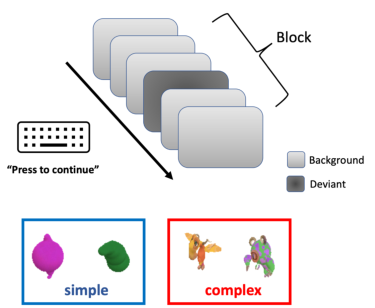
\includegraphics[width=\textwidth]{pokebaby_main_files/figure-latex/unnamed-chunk-7-1} 

}

\caption{Experimental design and examples of simple and complex stimuli. In each block, a deviant could appear on the second, fourth (as depicted here) or sixth trial or not at all. Stimuli within a block were either all simple or all complex.}\label{fig:unnamed-chunk-7}
\end{figure}

\hypertarget{procedure}{%
\subsubsection{Procedure}\label{procedure}}

The experiment was a web-based, self-paced visual presentation task. Participants were instructed to look at a sequence of animated creatures at their own pace and answer some questions throughout. On each trial, an animated creature showed up on the screen. Participants could press the down arrow to go to the next trial whenever they wanted to, after a minimum viewing time of 500 ms.

Each block consisted of six trials. Unbeknownst to the participants, each trial within the block was either a background trial or a deviant trial. One creature was assigned to be the `background' for each block, and was presented five or six times. If the block contained a deviant trial, then a new, unique, creature was presented on that trial. The deviant trial could appear at either the second, the fourth, or the sixth trial in the block, or not at all. The creatures presented in the deviant trials and background trials were matched for complexity. Each participant saw eight blocks in total, four with simple creatures and four with complex creatures, in random order across participants.

To test whether behavior was related to task demands, participants were randomly assigned to one of three attention check conditions, differing in the questions asked following each block: Curiosity, Memory, and Math. In the Curiosity condition, participants were asked to rate ``How curious are you about the creature?'' on a 5-point Likert scale. In the Memory condition, a forced-choice recognition question followed each block (``Have you seen this creature before?'', showing either a creature presented in the preceding block or a novel creature matched in complexity). In the Math condition, the participants were asked a simple arithmetic question (``What is 5 + 7?'') in a multiple-choice format.

To check if our complexity manipulation was successful, at the end of the eight blocks, participants were asked to rate the complexity of creatures they encountered on a 7-point Likert scale.

\hypertarget{participants}{%
\subsubsection{Participants}\label{participants}}

We recruited 449 participants (Age \emph{M} = 30.49; \emph{SD} = 9.74) on Prolific. They were randomly assigned to one of the three conditions of the experiment. Participants were excluded if they showed irregular reaction times (e.g.~three absolute deviations away from the median in the log-transformed space) or their responses in the filler tasks indicated low engagement with the experiment. All exclusion criteria were pre-registered. The final sample included 380 participants (Curiosity: \emph{N} = 143; Memory: \emph{N} = 98; Math: \emph{N} = 139).

\hypertarget{results}{%
\subsection{Results}\label{results}}

The sample size, methods, and main analyses were all pre-registered and are available at \url{https://aspredicted.org/3CR_VDR}. Data and analysis scripts are available at \url{https://github.com/anjiecao/pokebaby_CogSci2022}

We first checked whether the basic complexity manipulations were successful. Complex animated creatures were rated as more perceptually complex (\emph{M} = 4.63 ; \emph{SD} = 1.08) than the simple animated creatures (\emph{M} = 1.06; \emph{SD} = 1.06; \emph{p} \textless{} 0.001).

Next, we tested whether the task (Curiosity, Memory, or Math) affected reaction times in self-paced viewing (our measure of interest). There were no task effects so we averaged all results across the three conditions.

We were interested in whether our paradigm successfully captured the characteristic looking time patterns observed in infant literature: habituation (the decrease in looking time for a stimulus with repeated presentations), dishabituation (the increase in looking time to a new stimulus after habituated to one stimulus), and complexity effects (longer looking time for perceptually more complex stimuli). The visualization of our results suggests that we reproduce the phenomena qualitatively (Fig. 3, row 1). To evaluate the phenomena quantitatively, we ran a linear mixed effects model with maximal random effect structure. The predictors included in the model were a three-way interaction term between the trial number (modeled as an exponential decay; Kail, 1991), the type of trial (background vs.~deviant) and the complexity of the stimuli (simple vs.~complex). The model failed to converge, so we pruned the model following the pre-registered procedure. The final model included per-subject random intercepts. All predictors except for the three-way interaction were significant in the model (all \emph{p} \textless{} .001), providing a quantitative confirmation that our paradigm successfully captured the key looking time patterns: habituation (trial number), dishabituation (the deviant effect), and complexity (the stimulus complexity effect). We next tested whether we could capture these behavioral results using the RANCH model.

\hypertarget{model}{%
\section{Model}\label{model}}

RANCH treats the learning problem that participants face in our experiment as a form of Bayesian concept learning (Goodman, Tenenbaum, Feldman, \& Griffiths, 2008; Tenenbaum, 1999). In this setting, multiple noisy samples inform the learner's hypothesis about a probabilistic concept represented by a set of binary features (Figure 2). Like our participants, the model needs to decide at every step whether to keep looking at the current stimulus or terminate the trial by ``looking away''.

\begin{figure}[H]

{\centering 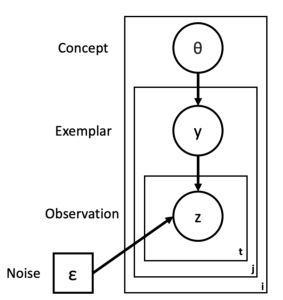
\includegraphics{pokebaby_main_files/figure-latex/unnamed-chunk-11-1} 

}

\caption{Graphical representation of RANCH. Circles indicate random variables. The square indicates fixed model parameters.}\label{fig:unnamed-chunk-11}
\end{figure}

The formulation of the learner as taking noisy samples from a stimulus allows us to do two things. First, we can explicitly model the learner's decision about when to stop sampling by asking the model to decide, after every sample, whether it wants to continue sampling from the same stimulus or not. This aspect of RANCH contrasts with previous models, which correlate information-theoretic measures to looking data overall (Kidd et al., 2012; Poli et al., 2020) but do not provide a mechanism for how these measures could control moment-to-moment sampling decisions. Second, a consequence of making a decision at every time step is that we can study the behavior of another information-theoretic measure: the model's expected information gain (EIG). EIG is commonly used in rational analyses of information-seeking behavior to assess whether information-seeking is optimal with respect to the learning task (Markant \& Gureckis, 2012; Oaksford \& Chater, 1994).

\hypertarget{model-definition}{%
\subsection{Model definition}\label{model-definition}}

In our setting, the goal is to learn a concept \(\theta\), which is a set of probabilities over independent binary features \(\theta_{1,2,..,n}\), where \(n\) is the number of features. \(\theta\) in turn generates exemplars \(y\): instantiations of \(\bar{\theta}\), where each feature \(y_{1,2,..,n}\) is present or absent. The weights on each feature \(\theta_i\) are sampled from a Beta prior, and individual exemplars \(y_i\) are distributed as a binomial with parameter \(\theta_i\), forming a conjugate Beta-Bernoulli distribution. Since the features are independent, this relationship holds for the entire concept \(\theta\).

To model the timecourse of attention, RANCH does not observe exemplars directly. Instead, it can observe repeated noisy samples \(\bar{z}\) from each exemplar. For any sample \(z\) from an exemplar \(y\) there is a small probability \(\epsilon\) that the observation is flipped and the feature is seen to be present when it was actually absent or vice versa. \(\epsilon\) is assumed to be unknown but to have a Beta prior; in practice, we integrate over all possible values of \(\epsilon\). Therefore, by making noisy observations \(\bar{z}\), RANCH obtains information about the true identity of the exemplar \(y\), and by extension, about the concept \(\bar{\theta}\). By Bayes' rule:

\begin{eqnarray}
P(\theta|\bar{z}) &= p(\bar{z}|y) p(y|\theta) p(\theta) / p(\bar{z})
\end{eqnarray}

To compute approximate posterior probability distributions during inference, we used a discrete grid approximation with a step size of .001 over both \(\theta\) and \(\epsilon\).

Upon observing a sample, RANCH then decides whether to keep sampling or not. We chose EIG from the next sample as the main linking hypothesis between the learned posterior and sampling choice.

RANCH computes EIG by iterating through each possible next observation and weighing the information gain from each observation by its posterior predictive probability \(p(z|\theta)\). We defined information gain as the KL between the hypothetical posterior after observing a future sample \(z_{t+1}\) and the current posterior (Baldi \& Itti, 2010):

\begin{eqnarray}
EIG(z_{t+1}) = \sum_{z_{t+1} \in [0,1]} p(z_{t+1}|\theta_t) * D_{KL}(\theta_{t+1} || p(\theta_t))
\end{eqnarray}

Finally, to get actual sampling behavior from the model, it has to convert EIG into a binary decision about whether to continue looking at the current sample, or to advance to the next trial. The model does so via a Luce choice between the EIG from the next sample and a constant ``environmental EIG'' that is assumed to be the amount of information to be gained via looking away from the stimulus.

\begin{eqnarray}
p(look away) = \frac{EIG(env)}{EIG(z_{t+1})+EIG(env)}
\end{eqnarray}

The basic structure of the model can be described in the following pseudocode:

\begin{algorithm}
  \caption*{RANCH model}\label{msn}
  \begin{algorithmic}
  \For{each exemplar y}
    \State{$sample \gets T$}
    \While{$sample$ take another sample z}
    \State{update posterior $P(\theta|z)$}
    \State{compute EIG of next sample $z_{t+1}$}
    \State{flip $coin$ with $p(lookaway) = \frac{EIG(env)}{EIG(z_{t+1})+EIG(env)}$}
    \If{$coin = T$}
    \State{$sample \gets F$}
    \EndIf
    \EndWhile
  \EndFor
\end{algorithmic}
  \end{algorithm}

\hypertarget{simulations}{%
\subsection{Simulations}\label{simulations}}

To model the behavioral experiment, we first represented the stimuli as binary-valued vectors indicating the presence (1) or absence (0) of each feature. All stimulus vectors were chosen to be length 6 to provide sufficient representational flexibility. Complex stimuli were represented as having three 1s and simple stimuli were represented as having one 1, with the rest of the features set to 0. Individual stimuli were then assembled into sequences to reflect the stimuli sequences in the behavioral experiment. For a particular sequence, we constructed the deviant stimulus based on the background stimulus to make sure that they were always maximally different and had the same number of features present.

Since the model makes stochastic choices about how many samples to take from each stimulus, behavior varies substantially across runs. Thus, we conducted 500 runs for each stimuli sequence and parameter value to obtain a reasonably precise estimate of the model's behavior.

\hypertarget{parameter-estimation}{%
\subsection{Parameter estimation}\label{parameter-estimation}}

We performed an iterative grid search in parameter space. We a priori constrained our parameter space on the prior beta distribution to have shape parameters \(\alpha_{\theta} > \beta_{\theta}\), which describe the prior beliefs as ``more likely to see the absence of a feature than the presence of a feature''. We then searched for the priors over the concept (\(\theta\)), the noise parameter that decides how likely a feature would be misperceived (\(\epsilon\)), and the constant EIG from the environment (\(EIG(env)\)). The prior over the noise parameter was fixed for all searches (\(\alpha_{\epsilon}\) = 1;\(\beta_{\epsilon}\) = 10). We selected the parameters that achieved the highest correlation with the behavioral data averaged across participants and blocks (\(\alpha_{\theta}\) = 1, \(\beta_{\theta}\) = 4, \(\epsilon\) = 0.065, \(EIG(env)\) = 0.01). No parameter regimes showed qualitatively different patterns, though the magnitude of dishabituation was strongly dependent on the priors over \(\theta\); a test of the generality of these specific parameter values is left for future work.

\hypertarget{results-1}{%
\subsection{Results}\label{results-1}}

\begin{figure}

{\centering 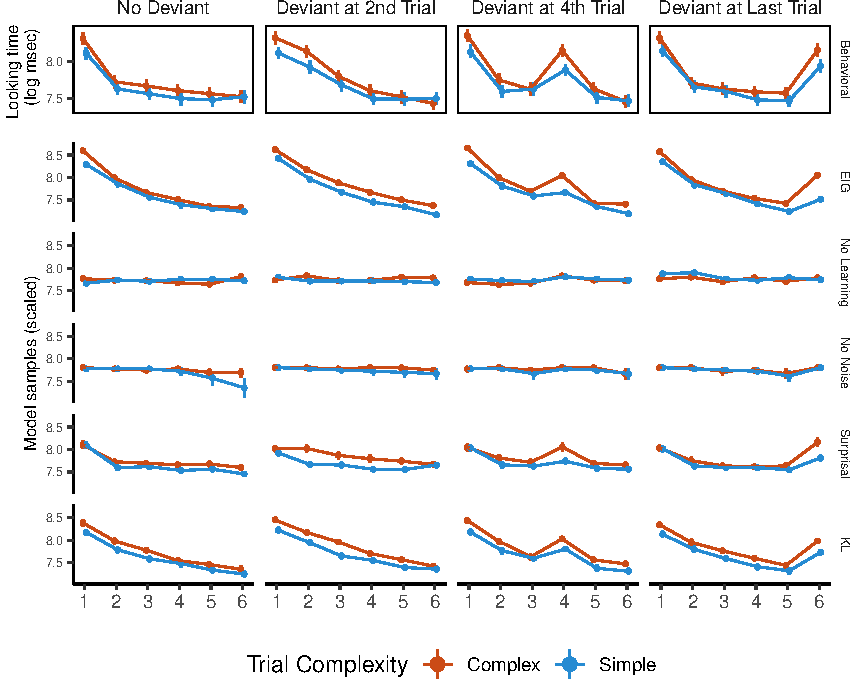
\includegraphics[width=\textwidth]{pokebaby_main_files/figure-latex/unnamed-chunk-12-1} 

}

\caption{The first row shows behavioral data. All models’ results were adjusted to match behavioral data’s scale and intercepts for easier comparisons. All results were log-transformed. Red lines indicate results for complex stimuli, and blue lines indicate results for simple stimuli.}\label{fig:unnamed-chunk-12}
\end{figure}

RANCH exhibited the main phenomena of interest, showing habituation, dishabituation, and complexity effects (Fig. 3, row 2). We also quantitatively explored the model by fitting the model results to the behavioral data (See Table 1, row 1). Overall RANCH achieved a good fit, though it did show a slightly more gradual habituation process than the behavioral data.

\begin{table}[tbp]

\begin{center}
\begin{threeparttable}

\caption{\label{tab:unnamed-chunk-13}Model fits}

\begin{tabular}{lll}
\toprule
Model Type (Linking Hypothesis) & \multicolumn{1}{c}{Pearson's r} & \multicolumn{1}{c}{RMSE}\\
\midrule
RANCH (EIG) & 0.92 [0.84, 0.96] & 0.19 [0.16, 0.24]\\
Baseline: No Learning & 0.21 [-0.09, 0.46] & 0.27 [0.23, 0.34]\\
Baseline: No Noise & 0.5 [0.36, 0.65] & 0.25 [0.21, 0.31]\\
RANCH (Surprisal) & 0.92 [0.86, 0.95] & 0.13 [0.11, 0.16]\\
RANCH (KL-divergence) & 0.93 [0.88, 0.96] & 0.12 [0.1, 0.15]\\
\bottomrule
\addlinespace
\end{tabular}

\begin{tablenotes}[para]
\normalsize{\textit{Note.} This table shows the correlations between the log-transformed model results and the log-transformed looking time data. The values in square brackets are 95\% confidence intervals. RANCH model implemented with the three different linking hypotheses showed similar performance with slight numerical differences and outperformed the baseline models.}
\end{tablenotes}

\end{threeparttable}
\end{center}

\end{table}

\hypertarget{alternative-models}{%
\section{Alternative Models}\label{alternative-models}}

\hypertarget{baseline-models}{%
\subsubsection{Baseline models}\label{baseline-models}}

We next wanted to test what aspects of the model are necessary to produce the phenomena. We focused on two assumptions: 1) the model makes decisions based on learning and 2) perception is noisy. We implemented lesioned baseline models corresponding to each assumption.

The first baseline model (No Learning) made random sampling decisions by drawing \(p(look away)\) from a uniform distribution between 0 and 1 at every time step. The second baseline model (No Noise) omitted the noisy sampling aspect of RANCH. We assumed that learning is free from perceptual noise, i.e.~that learners can observe the exemplars \(y\) directly. To do so, we set \(\epsilon\) to 0 and replaced the learner's beliefs about the true value of \(\epsilon\) with the assumption that perception was noiseless (for numerical stability we set the value to 0.000001 instead of 0). The baseline models used the parameters obtained from fitting the EIG model to the behavioral data.

The baseline models fit the data poorly (Table 1, row 2-3; Fig 3, row 3-4), suggesting that both learning and noisy perception are critical for modeling the phenomena of interest.

\hypertarget{alternative-linking-hypotheses}{%
\subsubsection{Alternative linking hypotheses}\label{alternative-linking-hypotheses}}

We also studied the behavior of RANCH using two other linking hypotheses, surprisal and Kullback-Leibler (KL) divergence. Both have been used in previous attempts to model infant looking behavior (Kidd et al., 2012; Poli et al., 2020) and to approximate EIG in the reinforcement learning literature (Kim, Sano, De Freitas, Haber, \& Yamins, 2020).

We implemented these by replacing \(EIG(z_{t+1})\) in Equation 2. Surprisal, formally described as \(-log(p(z|\theta))\), intuitively refers to how surprising an observation \(z\) is given the model's beliefs about \(\theta\) -- the intuition that surprising events should result in longer looking times has served as a foundational assumption in developmental psychology (Sim \& Xu, 2019). KL, formally described as \(\sum_{x \in X}{p(\theta = x|z) log \frac{p(\theta = x|z)}{p(\theta = x)}}\), measures how much the model changed to accommodate the most recent observation \(z\). The intuition behind using KL as a linking hypothesis is that, if one observation causes a large change, the next one might too, so continuing to sample is likely to be informative. We re-fit the free parameters (prior, noise and the environmental EIG) for these linking hypotheses to ensure a fair comparison.

In our experiment, the performance of surprisal and KL matched that of EIG (Table 1, row 4-5, Fig 3, row 5-6). To calculate EIG, the model needs to consider all combinations of possible features for the next observation and how informative they would be, a computation that can be intractable in richer environments. The similarity of model fits between EIG, surprisal and KL suggests that easier-to-compute metrics could be viable heuristics for choice behavior, at least in the current learning context.

\hypertarget{general-discussion}{%
\section{General discussion}\label{general-discussion}}

The current work aims to provide a computational model that can explain key phenomena observed in typical infant looking time paradigms: habituation, dishabituation, and how these are modified by stimulus complexity. RANCH assumes a rational learner that takes noisy perceptual samples from stimuli and makes sampling decisions based on EIG. We evaluated the model with adult looking time data collected from a paradigm that mirrors classic infant looking time paradigms, in which participants are learning about multi-feature concepts, and found that RANCH could successfully reproduce the patterns observed in behavioral data. By contrasting the model results with our baseline models, we showed that habituation, dishabituation, and complexity effects only arise in a learning model that takes into account the noisy nature of perception. Moreover, we found that, in the current learning context, other information theoretic quantities (surprisal and KL) are good proxies for the optimal linking hypothesis, EIG.

RANCH constitutes a significant step forward in the modeling of looking time in that it models the moment-to-moment decision making process of whether to keep sampling or look away. Previous approaches incremented time in steps of whole stimuli and therefore correlated information-theoretic variability in the stimulus sequence to look-away probability and looking time, rather than producing these behaviors endogenously. Our account of the sampling process depends on assuming that perception is noisy, which makes it necessary to take multiple samples from a stimulus until the information content of the stimulus has been learned sufficiently.

The similarity between model fits among models with different linking hypotheses highlights the significance of learning contexts. Our results should not be interpreted as evidence showing that the three linking hypotheses are indistinguishable across all learning contexts. Previous work has shown that adopting surprisal as learning policy can lead to undesirable behaviors in artificial agents (e.g.~``the white noise problem,'' Oudeyer et al., 2007). Moreover, the two alternative linking hypotheses are backward-looking metrics that utilize heuristics about the past to make decisions. This characteristic could constrain their application to situations in which the environment is stable and the cost of sampling is low. Since adult exploration is sensitive to environmental complexity, a forward-looking metric like EIG might be particularly suitable to predict behaviors in a more dynamic learning context (Dubey \& Griffiths, 2020; Vogelstein et al., 2022).

There are several limitations to our work. For our behavioral data, one concern is that adult looking time might not be driven by intrinsic interest to the same degree as infant looking time. Rather, they might be driven by task-preparation. However, across the three conditions with different cover tasks, we found no differences in looking time patterns. In regards to the model, a few concerns can be raised. First, the current stimulus representation is oversimplified, using an unweighted collection of binary features. Future research could apply RANCH to stimulus representations generated from a perceptual model. Second, RANCH assumes that the EIG from the environment is a constant throughout the experiment, but one can argue that environmental EIG might increase as the experiment progresses (e.g.~the longer you have not attended to the things in your surroundings, the more they may have changed in the meantime). While implementing more sophisticated assumptions could potentially explain additional variance in the data, our current work suggests that even a simple rational learner that takes noisy samples from a set of independent binary features is capable of explaining key phenomena.

Our ultimate goal is to provide a rational learner model that can account for information-seeking behaviors reflected in infants' looking time. Here we have shown that a simple model of learning from sampling can reproduce habituation, dishabituation, and complexity effects. Moving forward, we aim to capture and explain more contentious phenomena documented in the infant looking time literature such as familiarity preferences and age effects (Hunter \& Ames, 1988). Our ongoing work with infants will eventually enable us to evaluate our model with developmental data. When combined with adult results, the data and model will provide insights into the general mechanisms through which learners decide what to look at, and when to stop looking.

\hypertarget{references}{%
\section{References}\label{references}}

\hypertarget{refs}{}
\begin{CSLReferences}{1}{0}
\leavevmode\vadjust pre{\hypertarget{ref-aslin2007s}{}}%
Aslin, R. N. (1991). Development of processing speed in childhood and adolescence. \emph{Advances in Child Development and Behavior}, \emph{23}, 151--185.

\leavevmode\vadjust pre{\hypertarget{ref-baillargeon1985object}{}}%
Baillargeon, R., Spelke, E. S., \& Wasserman, S. (1985). Object permanence in five-month-old infants. \emph{Cognition}, \emph{20}(3), 191--208.

\leavevmode\vadjust pre{\hypertarget{ref-baldi2010bits}{}}%
Baldi, P., \& Itti, L. (2010). Of bits and wows: A bayesian theory of surprise with applications to attention. \emph{Neural Networks}, \emph{23}(5), 649--666.

\leavevmode\vadjust pre{\hypertarget{ref-bitzer2014perceptual}{}}%
Bitzer, S., Park, H., Blankenburg, F., \& Kiebel, S. J. (2014). Perceptual decision making: Drift-diffusion model is equivalent to a bayesian model. \emph{Frontiers in Human Neuroscience}, \emph{8}, 102.

\leavevmode\vadjust pre{\hypertarget{ref-callaway2021fixation}{}}%
Callaway, F., Rangel, A., \& Griffiths, T. L. (2021). Fixation patterns in simple choice reflect optimal information sampling. \emph{PLoS Computational Biology}, \emph{17}(3), e1008863.

\leavevmode\vadjust pre{\hypertarget{ref-carey2009}{}}%
Carey, S. (2009). \emph{The origin of concepts}. Oxford University Press.

\leavevmode\vadjust pre{\hypertarget{ref-colombo2009infant}{}}%
Colombo, J., \& Mitchell, D. W. (2009). Infant visual habituation. \emph{Neurobiology of Learning and Memory}, \emph{92}(2), 225--234.

\leavevmode\vadjust pre{\hypertarget{ref-dubey2020reconciling}{}}%
Dubey, R., \& Griffiths, T. L. (2020). Reconciling novelty and complexity through a rational analysis of curiosity. \emph{Psychological Review}, \emph{127}(3), 455.

\leavevmode\vadjust pre{\hypertarget{ref-fantz1963pattern}{}}%
Fantz, R. L. (1963). Pattern vision in newborn infants. \emph{Science}, \emph{140}(3564), 296--297.

\leavevmode\vadjust pre{\hypertarget{ref-frank2017collaborative}{}}%
Frank, M. C., Bergelson, E., Bergmann, C., Cristia, A., Floccia, C., Gervain, J., et al.others. (2017). A collaborative approach to infant research: Promoting reproducibility, best practices, and theory-building. \emph{Infancy}, \emph{22}(4), 421--435.

\leavevmode\vadjust pre{\hypertarget{ref-goodman2008rational}{}}%
Goodman, N. D., Tenenbaum, J. B., Feldman, J., \& Griffiths, T. L. (2008). A rational analysis of rule-based concept learning. \emph{Cognitive Science}, \emph{32}(1), 108--154.

\leavevmode\vadjust pre{\hypertarget{ref-haber2018learning}{}}%
Haber, N., Mrowca, D., Fei-Fei, L., \& Yamins, D. L. (2018). Learning to play with intrinsically-motivated self-aware agents. \emph{arXiv Preprint arXiv:1802.07442}.

\leavevmode\vadjust pre{\hypertarget{ref-haith1980rules}{}}%
Haith, M. M. (1980). \emph{Rules that babies look by: The organization of newborn visual activity}. Lawrence Erlbaum Associates.

\leavevmode\vadjust pre{\hypertarget{ref-haith1998put}{}}%
Haith, M. M. (1998). Who put the cog in infant cognition? Is rich interpretation too costly? \emph{Infant Behavior and Development}, \emph{21}(2), 167--179.

\leavevmode\vadjust pre{\hypertarget{ref-hills2015exploration}{}}%
Hills, T. T., Todd, P. M., Lazer, D., Redish, A. D., Couzin, I. D., Group, C. S. R., et al. (2015). Exploration versus exploitation in space, mind, and society. \emph{Trends in Cognitive Sciences}, \emph{19}(1), 46--54.

\leavevmode\vadjust pre{\hypertarget{ref-hunter1988multifactor}{}}%
Hunter, M. A., \& Ames, E. W. (1988). A multifactor model of infant preferences for novel and familiar stimuli. \emph{Advances in Infancy Research}.

\leavevmode\vadjust pre{\hypertarget{ref-kersten2004object}{}}%
Kersten, D., Mamassian, P., \& Yuille, A. (2004). Object perception as bayesian inference. \emph{Annu. Rev. Psychol.}, \emph{55}, 271--304.

\leavevmode\vadjust pre{\hypertarget{ref-kidd2012goldilocks}{}}%
Kidd, C., Piantadosi, S. T., \& Aslin, R. N. (2012). The goldilocks effect: Human infants allocate attention to visual sequences that are neither too simple nor too complex. \emph{PloS One}, \emph{7}(5), e36399.

\leavevmode\vadjust pre{\hypertarget{ref-kim2020active}{}}%
Kim, K., Sano, M., De Freitas, J., Haber, N., \& Yamins, D. (2020). Active world model learning with progress curiosity. \emph{International Conference on Machine Learning}, 5306--5315. PMLR.

\leavevmode\vadjust pre{\hypertarget{ref-liquin2021developmental}{}}%
Liquin, E. G., Callaway, F., \& Lombrozo, T. (2021). Developmental change in what elicits curiosity. \emph{Proceedings of the Annual Meeting of the Cognitive Science Society}, \emph{43}.

\leavevmode\vadjust pre{\hypertarget{ref-markant2012does}{}}%
Markant, D., \& Gureckis, T. (2012). Does the utility of information influence sampling behavior? \emph{Proceedings of the Annual Meeting of the Cognitive Science Society}, \emph{34}.

\leavevmode\vadjust pre{\hypertarget{ref-oakes2010using}{}}%
Oakes, L. M. (2010). Using habituation of looking time to assess mental processes in infancy. \emph{Journal of Cognition and Development}, \emph{11}(3), 255--268.

\leavevmode\vadjust pre{\hypertarget{ref-oaksford1994rational}{}}%
Oaksford, M., \& Chater, N. (1994). A rational analysis of the selection task as optimal data selection. \emph{Psychological Review}, \emph{101}(4), 608.

\leavevmode\vadjust pre{\hypertarget{ref-oudeyer2007intrinsic}{}}%
Oudeyer, P.-Y., Kaplan, F., \& Hafner, V. V. (2007). Intrinsic motivation systems for autonomous mental development. \emph{IEEE Transactions on Evolutionary Computation}, \emph{11}(2), 265--286.

\leavevmode\vadjust pre{\hypertarget{ref-pirolli1999information}{}}%
Pirolli, P., \& Card, S. (1999). Information foraging. \emph{Psychological Review}, \emph{106}(4), 643.

\leavevmode\vadjust pre{\hypertarget{ref-poli2020infants}{}}%
Poli, F., Serino, G., Mars, R., \& Hunnius, S. (2020). Infants tailor their attention to maximize learning. \emph{Science Advances}, \emph{6}(39), eabb5053.

\leavevmode\vadjust pre{\hypertarget{ref-sim2019another}{}}%
Sim, Z. L., \& Xu, F. (2019). Another look at looking time: Surprise as rational statistical inference. \emph{Topics in Cognitive Science}, \emph{11}(1), 154--163.

\leavevmode\vadjust pre{\hypertarget{ref-tenenbaum1999bayesian}{}}%
Tenenbaum, J. B. (1999). Bayesian modeling of human concept learning. \emph{Advances in Neural Information Processing Systems}, 59--68.

\leavevmode\vadjust pre{\hypertarget{ref-vogelstein2022prospective}{}}%
Vogelstein, J. T., Verstynen, T., Kording, K. P., Isik, L., Krakauer, J. W., Etienne-Cummings, R., et al.others. (2022). Prospective learning: Back to the future. \emph{arXiv Preprint arXiv:2201.07372}.

\end{CSLReferences}


\end{document}
